\subsection{Resultados obtenidos por el prototipo a 50.00 C}

\begin{figure}[H]
	\centering
	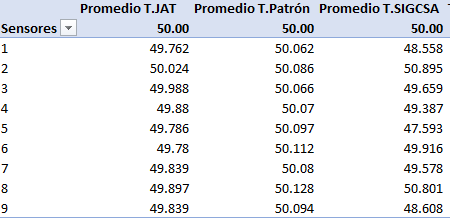
\includegraphics[width=0.5\linewidth]{resultados9.png}
	\caption{Tabla de Promedios de Temperaturas de prototipo y termómetros a 30.00 C}
\end{figure}

\par \noindent 
Los resultados obtenidos por las calibraciones, ver Anexo 4 , son utilizados para calcular la temperatura promedio del termómetro patrón, los nueve termómetros de campo de SIGCSA y los sensores de temperatura del prototipo, ver figura 4.9 y con estos valores podemos realizar la siguiente gráfica:

\begin{figure}[H]
	\centering
	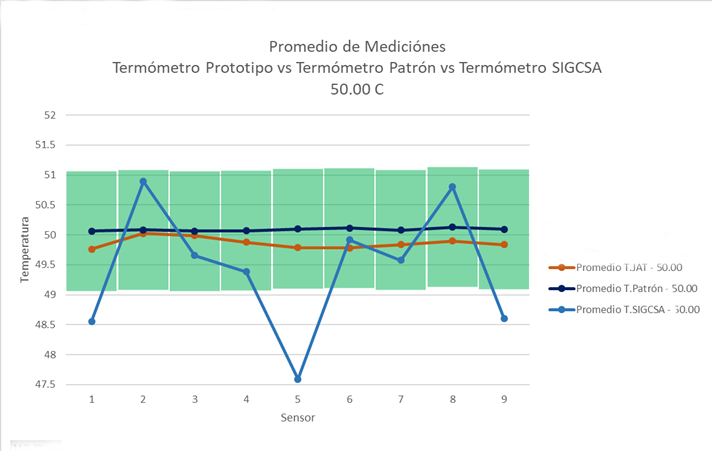
\includegraphics[width=0.6\linewidth]{resultados10.png}
	\caption{Grafica de Promedios de Temperaturas de prototipo y termómetros a 30.00 C}
\end{figure}

\par \noindent
En la última gráfica, figura 4.10. Dos de los termómetros de campo previamente mencionados salen del error máximo permitido (1 y 9) y el termómetro de campo 6 se aleja cada vez más del patrón. Los termómetros de campo 2 y 8 se encuentran muy cercanos del error máximo. Los sensores de temperatura del prototipo aún siguen manteniendo un margen de error aceptable; sin embargo, ya a esta temperatura podemos encontrar un aumento del error de medición con respecto al patrón específicamente en el sensor 1 y 5.
